%%=============================================================================
%% Shortlist
%%=============================================================================

\chapter{\IfLanguageName{dutch}{Selectie van tools}{Selection of tools}}
\label{ch:shortlist}
Hierna volgen enkele beslissingen rond de gebruikte tools en technologie\"en in het technische luik van deze paper.
De vereisten van de opdrachtgever staan hierbij centraal zoals besproken in de~\nameref{sec:onderzoeksdoelstelling}.
Daarnaast komt ook een korte uitleg rond de keuze voor het te testen fitnessinstrument aan bod.
Het volgende hoofdstuk beschrijft vervolgens de uitwerking van dit luik met de gekozen tools in de vorm van een proof-of-concept.

\section{Android-app met Jetpack Compose}
\label{sec:keuze-framework-voor-android-app}
Een van de vereisten van deze bachelorproef is het frictieloos aanroepen van de achterliggende service.
De proef is erop gericht om de gebruiker met een simpele foto alle functionaliteiten te kunnen gebruiken.
Hierdoor zijn native en cross-platform applicaties meer geschikt boven progressive web apps.
Native en cross-platform raamwerken zoals Jetpack Compose en Flutter bieden het gebruik van bestaande tools specifiek voor het besturingssysteem om foto's te maken en door te sturen.
Gebruikers zullen daarmee de Android app kunnen gebruiken zoals ze eender welke app zouden gebruiken om foto's op te laden, zij het Instagram of Google Photos.

\subsection{Motivering voor Jetpack Compose}
\label{subsec:motivering-voor-jetpack-compose}
Jetpack Compose biedt een oplossing voor Android-specifieke mobiele applicaties en wordt daardoor als een native raamwerk aanschouwd.
Bovendien past het beter bij de keuze voor Quarkus als achterliggend raamwerk, gezien beiden gebruik maken van het Gradle bouwsysteem en het Java ecosysteem.
Een bijkomend voordeel is de betere performantie doordat applicaties specifiek voor het Android besturingssysteem gemaakt zijn, wat de vereiste van een frictieloze gebruikerservaring garandeert.

\section{Achterliggende service met Quarkus}
\label{sec:keuze-framework-voor-back-end}
Quarkus is een open source raamwerk bovenop het Java ecosysteem dat talloze functionaliteiten biedt aan softwareontwikkelaars om Java applicaties uit te werken.
RedHat, een dochteronderming van IBM dat zich richt op het toegankelijk maken van open-source software, sponsort en ondersteunt dit initiatief.
Bovendien dragen ontwikkelaars binnen RedHat bij aan het project met de ontwikkeling van Mandrel, een distributie van GraalVM specifiek voor de vereisten van Quarkus.
Mede door deze ondersteuning kent Quarkus een penetratie in het door Java Spring-gedomineerde landschap van Java raamwerken.

\subsection{Modern raamwerk}
\label{subsec:modern-raamwerk}
Quarkus is een modern raamwerk ontstaan in 2019 dat verder bouwt op industriestandaarden zoals de Java Context~\& Dependency Injection CDI (CDI) en Persistence API (JPA) standaarden.
Hierdoor is het makkelijk te interpreteren en verder op te bouwen voor bestaande Java-ontwikkelaars met expertise in back-end ontwikkeling.
Bovendien heeft Quarkus het voordeel om deze standaarden te implementeren volgens hedendaagse vereisten met kennis opgedaan uit oudere raamwerken zoals Java Spring en Jakarta EE\@.
Met een focus op Kubernetes en de bijkomende \textit{Dev Services} wilt Quarkus zich differentiëren binnen het Java landschap.

\subsection{Quarkus Dev Services}
\label{subsec:quarkus-dev-services}
Aan de hand van~\autocite{Quarkus} ontstaat de mogelijkheid om op een snelle, iteratieve manier voort te bouwen zonder initiële configuratie.
Zolang er geen bijkomende configuratie van afhankelijke instanties van software aanwezig is, bijvoorbeeld de login details van een databank, voorziet Quarkus van deze instanties.
In het geval van de MariaDB databank, die gebruikt zal worden om de geschiedenis van gebruikers op te slaan, wordt daarbij achterliggend een Testcontainer opgestart.
Testcontainers draaien op Docker, een technologie die zich richt op het draaien van software op een platform-agnostische manier, wat verder aan bod komt in subsectie~\ref{subsec:docker}.

\subsection{Quarkus AI met Langchain4j}
\label{subsec:quarkus-ai-met-langchain4j}
Langchain4j is de Java-implementatie van Langchain, een raamwerk dat het communiceren met grote taalmodellen vermakelijkt.
Het is best te vergelijken met Java Hibernate, de industriestandaard raamwerk om het communiceren met achterliggende databanken toegankelijker te maken~\autocite{Langchain4j}.
Quarkus AI bouwt hierop verder door een Langchain4j integratie te voorzien voor Quarkus applicaties om grote taalmodellen toegankelijk te maken.
De situering van deze extensie is zichtbaar in afbeelding~\ref{fig:quarkus-ai}.

\begin{figure}[H]
    \begin{center}
        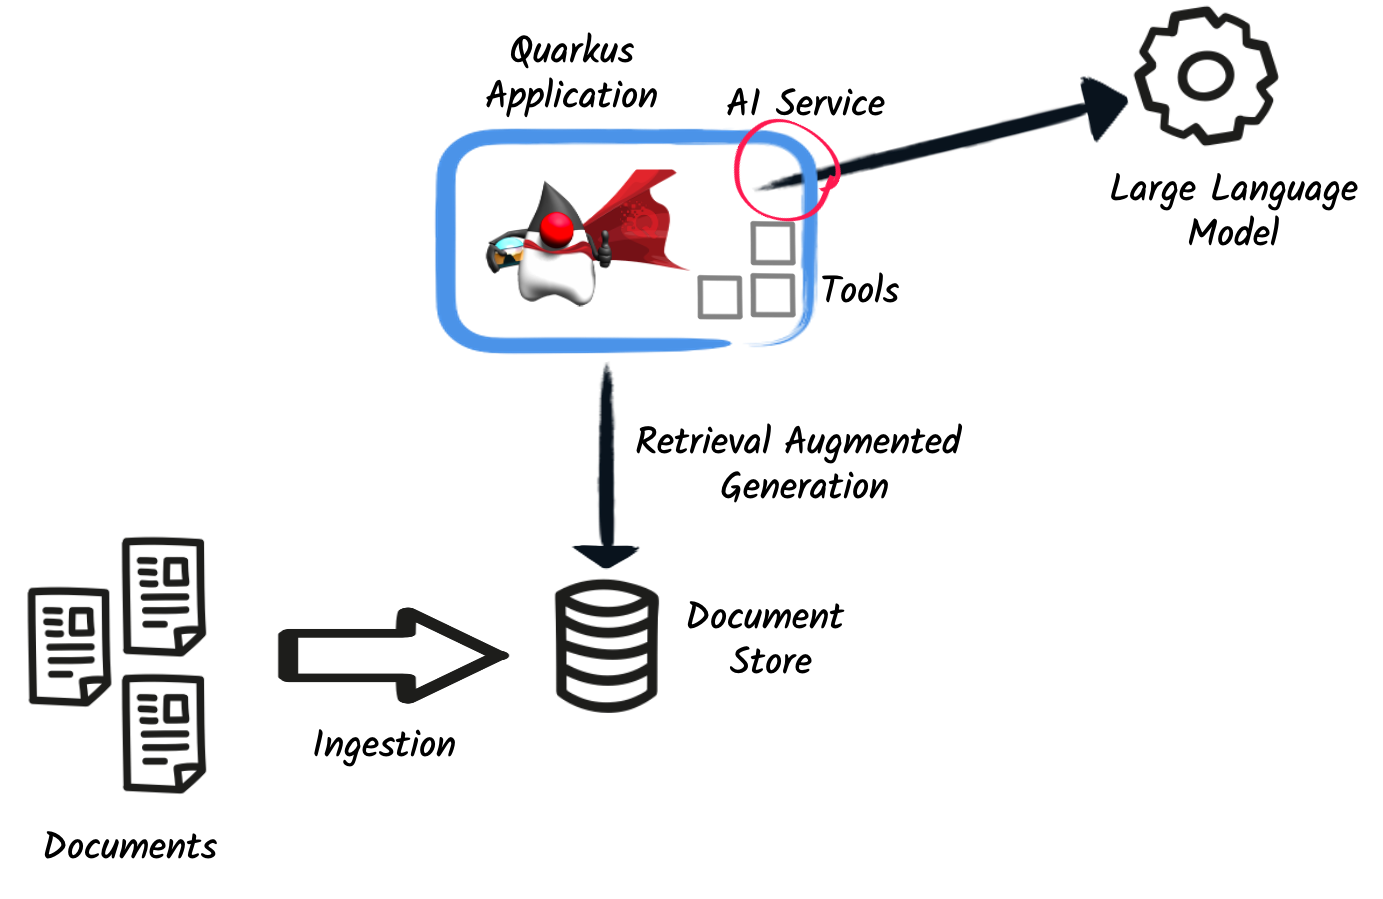
\includegraphics[scale=0.45]{images/quarkus-ai-visualisation}
        \caption{Quarkus AI is een dienst waarmee Quarkus applicaties kunnen communiceren met grote taalmodellen. De document store stelt hierbij de databank voor met de geschiedenis van gebruikers in het opvragen van suggesties rond fitnesstoestelen.~\autocite{Lowe2004}}
        \label{fig:quarkus-ai}
    \end{center}
\end{figure}

\section{Artificiële intelligentie met Vertex AI}
\label{sec:keuze-ai-platform}
Multimodale taalmodellen vereisen hoge rekenkracht om taken uit te voeren, hierdoor worden deze gebruikt via bestaande cloudinfrastructuur zoals Microsoft Azure en Amazon Web Services.
Met de vereiste om een kostenefficiënte oplossing uit te werken komt Google Cloud naar voren als platform.
Vertex AI, een dienst binnen Google Cloud, biedt daarbij bestaande taalmodellen met voorafgetrainde datasets en infrastructuur om zelf datasets te trainen.

\subsection{Gemini 1.5 Pro}
\label{subsec:gemini-1.5-pro}
Gemini, het Google equivalent van OpenAI's GPT en Meta's Llama, biedt verschillende modellen voor gebruikers van Vertex AI\@.
Versie 1.5 Pro is daarbij het meeste geschikt voor de proof-of-concept, gezien het zowel computer visie als generatieve AI biedt in één oplossing.
Het model laat toe om te specifiëren hoe betrouwbaar de resultaten horen te zijn, wat een belangrijk aspect is voor het voorstellen van suggesties aan cliënten van personal trainers.
Tot slot kan het model aangeroepen worden vanuit de Quarkus LangChain4j extensie.

\section{Build tool}
\label{sec:build-tool}
Moderne software projecten maken tegenwoordig gebruik van een \textit{build tool}, wat helpt bij vele taken binnen het ontwikkelingsproces.
Bovendien is dit een vereiste voor complexere applicaties waar enkele tussenstappen vereist zijn, zoals bij het bouwen van een Android-applicatie.
Eveneens vergemakkelijkt het gebruik van een bouwsysteem om de proof-of-concept reproduceerbaar te houden.

\subsection{Motivering}
\label{subsec:voordelen-van-een-build-tool}
\textcite{Kandhway2019}~beschrijven de vijf grootste voordelen van het gebruiken van een build tool:
\begin{itemize}
    \item \textbf{Het automatiseert het bouwproces van software.}
    Software moet eerst gecompileerd worden om leesbaar en uitvoerbaar te zijn door een machine.
    Dit is automatiseerbaar aan de hand van een build tool, wat zal helpen bij het~\nameref{sec:reproduceren-van-de-proof-of-concept}.
    \item \textbf{Het vergemakkelijkt het beheren van afhankelijkheden.}
    De achterliggende Quarkus service en de Android app zullen gebruik maken van libraries om het ontwikkelingsproces te vereenvoudigen.
    Een voorbeeld hiervan is het gebruik van de Quarkus REST-extensie, wat het verwerken van appgebruikers' verzoeken versoepelt.
    \item \textbf{Het verzekert het correct uitvoeren van het bouwproces.}
    Het bouwproces bestaat uit verschillende stappen die ondergaan moeten worden.
    Een build tool helpt hierbij om sommige stappen voor ons te bepalen, zoals de volgorde waarin afhankelijkheden inladen.
    \item \textbf{Het bespaart tijd door taken in parallel uit te voeren.}
    De build tool splitst taken op om gelijktijdig uit te voeren.
    Dit versnelt het bouwproces.
    \item \textbf{Het is een vereiste voor het toepassen van continuous integration.}
    \textit{Continuous integration} maakt het mogelijk om vooraf gedefinieerde bouwprocessen te lanceren eens er nieuwe code beschikbaar komt.
\end{itemize}

\subsection{Gradle als buildtool}
\label{subsec:gradle}
Binnen het Java-ecosysteem staan Apache Maven en Gradle centraal als build tools.
Bij sommige oudere applicaties is het Ant-bouwsysteem nog in gebruik.
Het Kotlin-ecosysteem kent de voorkeur naar Maven en Gradle gezien haar oorspronkelijk ontwerp om interoperabiliteit met Java te verzekeren.
Google, de ontwikkelaars achter het Jetpack Compose framework en het Android besturingssysteem, hebben ervoor gekozen om uitsluitend met Gradle te werken wegens de beperktheid van Maven op vlak van bouwprocessen opstellen.
Met de keuze voor Jetpack Compose zoals besproken in~\ref{sec:keuze-framework-voor-android-app} zal daarmee ook gebruik gemaakt worden van Gradle voor de achterliggende Quarkus service.
De reden hiervoor is om het bouwproces zo gestroomlijnd en consistent mogelijk te houden tussen de te ontwikkelende platformen, de visualisatie van dit bouwproces is te zien in afbeelding~\ref{fig:visualisatie-gradle-bouwproces}.
Een bijkomend voordeel is de mogelijkheid om de Kotlin-syntax te gebruiken binnen Gradlebestanden, wat het meer consistent maakt met de syntax van de Quarkus en Jetpack Compose applicaties.
\begin{figure}[H]
    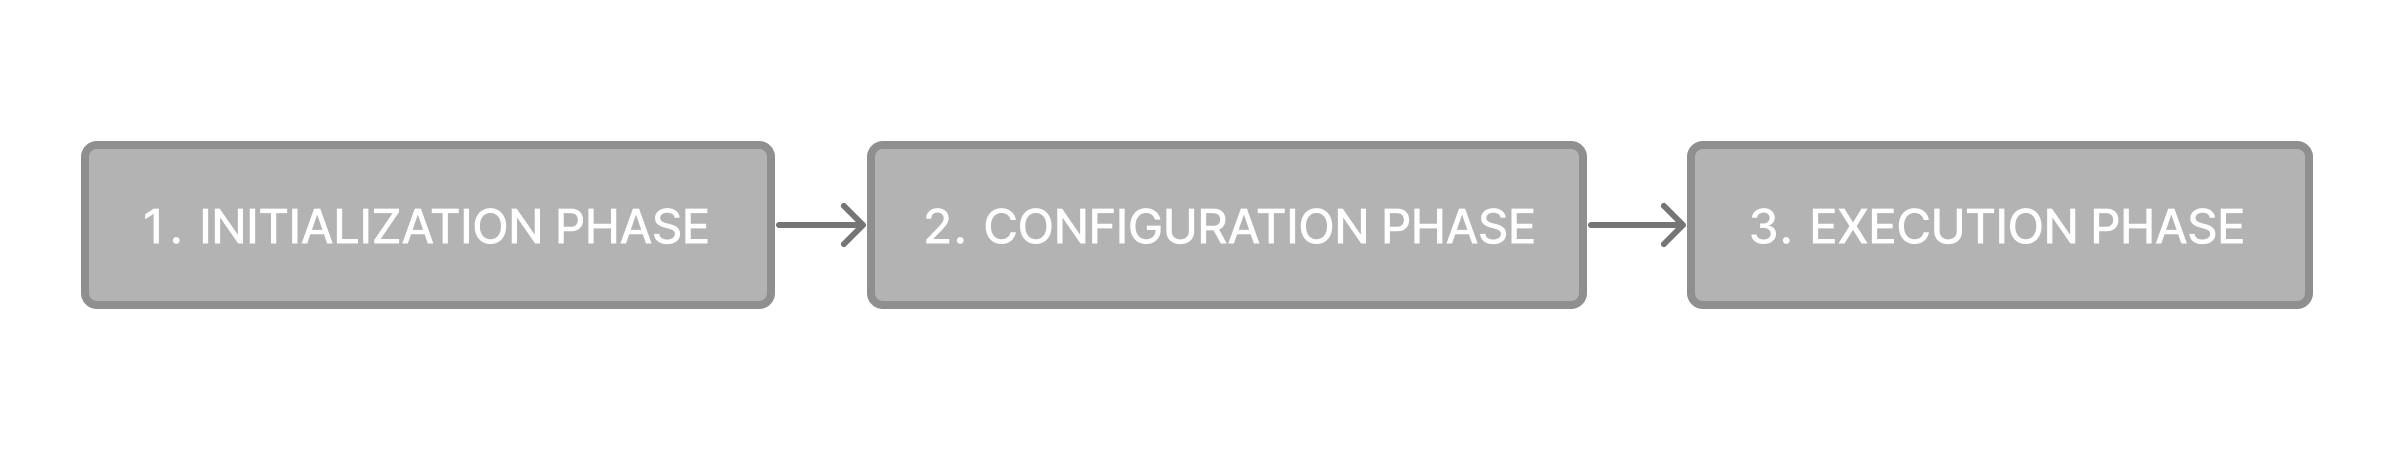
\includegraphics[width=1\linewidth]{images/gradle-buildprocess}
    \caption{De drie stappen in het Gradle bouwproces~\autocite{Gradle}}
    \label{fig:visualisatie-gradle-bouwproces}
\end{figure}

\section{Gekozen fitnessinstrument}
\label{sec:gekozen-fitnessinstrument}
Om de computer visie mogelijkheden uit testen zal gebruik gemaakt worden van afbeeldingen met dumbbells.
Dumbbells zijn vrije gewichten die in de hand vastgenomen kunnen worden.
Sporters gebruiken deze gewichten voornamelijk voor krachttraining en functionele training.
Deze activiteiten zijn populair onder sporters volgens een opmeting van~\textcite{Thompson2022}.
Bovendien zijn er vele ontwerpen van dumbbells in gebruik met of zonder gewichtsindicatie, wat een toegevoegde waarde biedt op het uittesten van de computer visie mogelijkheden.